\clearpage
\setcounter{page}{1}
\maketitlesupplementary

\section{Implementation Details}
\label{app:implementation_details}


\paragraph{Short-video segmentation.} To optimize training time, we pre-process all data once prior to pre-training. Specifically, for each dataset, the process outlined in \cref{subsec:short_video_representation} is applied only once. This ensures efficient handling of video inputs during the training phase.

\paragraph{Architectural design.} 
We adopt an asymmetric encoder-decoder architecture inspired by~\cite{he2022masked}. The encoder processes only the visible, unmasked tokens from the video input. Positional embeddings are added to each token to encode temporal relationships. The embedded tokens are then passed through a Transformer encoder with $K$ layers, where each layer includes a multi-head self-attention mechanism, a multi-layer perceptron (MLP), and LayerNorm. Unlike ViT architectures designed for fixed-size inputs, such as images, our encoder accommodates varying input lengths, enabling it to handle videos of arbitrary durations. Mask tokens are not used during this stage, ensuring computational efficiency by focusing exclusively on visible tokens.

After the encoder processes the visible tokens, the decoder reconstructs the full sequence by introducing shared, learned mask tokens to replace the missing inputs. These mask tokens are inserted at their respective positions in the sequence. To ensure that the mask tokens carry information about their temporal location, positional embeddings are applied to all tokens in the decoder input, including the mask tokens. Without these positional embeddings, the mask tokens would have no information about their location in the video. The decoder processes the full sequence through a series of Transformer layers. Following~\cite{he2022masked}, it is designed to be shallower than the encoder to maintain computational efficiency while providing accurate reconstructions.

To manage videos of varying lengths, we adapt sequence-processing techniques from BERT~\cite{devlin2019bert}. Each sequence of short-video embeddings is capped at 256 tokens, with shorter sequences padded using a special \texttt{[PAD]} token. During the self-attention process, an attention mask prevents these padding tokens from influencing training. This design ensures that the model maintains computational efficiency while supporting inputs of arbitrary length. Practically, our framework allows for increasing the maximum token limit, enabling the processing of even longer videos. However, since the benchmark datasets used in this study do not exceed 20 minutes, we leave such extensions for future exploration.

Finally, during pre-training, an auxiliary \texttt{[CLS]} token is appended to the input sequence in the encoder. This token serves as a representation of the entire video sequence and is specifically used for downstream tasks, such as classification. In attentive probing fine-tuning, this \texttt{[CLS]} token is adapted to generate task-specific predictions.


\begin{table}[t]
    \caption{\textbf{Pre-training setting.}}
    \vspace{-1.5em}
    \begin{center}
    \small
        \begin{tabular}{l|c}
            \hline
            
            \hline
            
            \hline\\[-3mm]
            \textbf{Config} & \textbf{Value } \\
            \hline
            optimizer & AdamW \\
            base learning rate & 1.5e-4 \\
            weight decay & 0.05 \\
            optimizer momentum & $\beta_1, \beta_2{=}0.9, 0.95$ \\
            batch size & 16 \\
            learning rate schedule & cosine decay \\
            warmup epochs & 40 \\
            epochs  & 150 \\
            number of tokens & 256 \\ 
            short video length & 5 sec \\ 
            \hline 
            
            \hline
            
            \hline
        \end{tabular}

    \end{center}
\vspace{-1.2em}
\label{tab:hyperparams_pretrain}
\vspace{1.5em}
\end{table}


\begin{table}[t]
    \caption{\textbf{Linear probing setting.}}
    \vspace{-1.5em}
    \begin{center}
    \small
        \begin{tabular}{l|c}
            \hline
            
            \hline
            
            \hline\\[-3mm]
            \textbf{Config} & \textbf{Value } \\
            \hline
            optimizer & Adam \\
            base learning rate & 1e-4 \\
            
            optimizer momentum & $\beta_1, \beta_2{=}0.9, 0.999$ \\
            batch size & 16 \\
            epochs  & 30 \\
            \hline 
            
            \hline
            
            \hline
        \end{tabular}
    \end{center}
\vspace{-1.2em}
\label{tab:hyperparams_lp}
\vspace{1.5em}
\end{table}


\begin{table}[t]
    \caption{\textbf{Attentive probing setting.}}
    \vspace{-1.5em}
    \begin{center}
    \small
        \begin{tabular}{l|c}
            \hline
            
            \hline
            
            \hline\\[-3mm]
            \textbf{Config} & \textbf{Value } \\
            \hline
            optimizer & Adam \\
            learning rate & 1e-3 \\
            learning rate schedule & ExponentialLR, $\gamma{=}0.9$ \\
            optimizer momentum & $\beta_1, \beta_2{=}0.9, 0.999$ \\
            batch size & 16 \\
            epochs  & 20 \\
            \hline 
            
            \hline
            
            \hline
        \end{tabular}
    \end{center}
\vspace{-1.2em}
\label{tab:hyperparams_ap}
\vspace{-0.5em}
\end{table}


\begin{table*}[t]
    \caption{\textbf{Additional LVU benchmark results.} In the main paper, we provided the average Top-1 accuracy results obtained by LV-MAE with linear probing (LP) and attentive probing (AP) with random masking. Here, we provide extended results per task. Masking indicates the masking technique that was applied. ``Dir.'' and ``Rel.'' refer to ``Director'' and ``Relationship,'' respectively.}
    \label{tab:lvu_benchmark_app}
    \centering
    \small
    \setlength{\tabcolsep}{6.5pt}
    \begin{tabular}[t]{l|c|cccc|ccc|c}
            \hline 
            
            \hline
            
            \hline
        \multirow{2}*{\textbf{Method}} & \multirow{2}*{\textbf{Masking}} & \multicolumn{4}{c|}{\textbf{Metadata $\uparrow$}} & \multicolumn{3}{c|}{\textbf{Content $\uparrow$}} & \multirow{2}*{\textbf{Avg.}} \\
        & & \textbf{Dir.} & \textbf{Genre} & \textbf{Writer} & \textbf{Year} & \textbf{Scene} & \textbf{Speak} & \textbf{Rel.} & \\
        \hline
        $\text{LV-MAE}_{\text{InternVideo2}}$(LP)  & Semantic & 55.14 &  58.56 & 49.40 & 43.26 & 72.84 & 37.77 & 51.22 & 52.60 \\
        $\text{LV-MAE}_{\text{InternVideo2}}$(LP)  & Random & 57.01 &  57.36 & 52.38 & 49.65 & 70.37 & 39.89 & 48.78 & 53.63 \\
        $\text{LV-MAE}_{\text{InternVideo2}}$(AP) & Random & 54.21 &  66.95 & 55.36 & 56.03 & 80.25 & 42.55 & 53.66 & 58.43 \\
        $\text{LV-MAE}_{\text{LanguageBind}}$(LP)  & Semantic & 71.03 & 67.47 & 54.76 & 53.90 & 67.90 & 42.02 & 56.09 & 59.02 \\
        $\text{LV-MAE}_{\text{LanguageBind}}$(LP)  & Random & 71.96 & 67.12 & 55.36 & 53.19 & 71.60 & 37.76 & 51.22 & 58.32 \\
        $\text{LV-MAE}_{\text{LanguageBind}}$(AP)  & Random & 78.50 & 69.17 & 60.12 & 61.70 & 72.84 & 39.36 & 56.09 & 62.54 \\
            \hline 
            
            \hline
            
            \hline
    \end{tabular}
\end{table*}



\paragraph{Pre-training hyperparameters.} 
Our pre-training hyperparameters are detailed in Table~\ref{tab:hyperparams_pretrain}. We closely follow the hyperparameter settings from~\cite{he2022masked} with a few adjustments. Specifically, we use a smaller batch size and reduce the number of epochs during pre-training. We set the limit for the number of tokens to 256. Finally, we set the short video segment length to five seconds.
The choice of a five-second segment length balances two considerations: it is short enough to capture low-level spatiotemporal patterns effectively using an off-the-shelf frozen model and sufficiently long to reduce the number of tokens required for longer videos. In future work, we plan to analyze the impact of segment lengths (e.g., 10–15 seconds) on performance, as longer segments could offer greater efficiency for processing extended videos. However, this may risk reduced performance from the frozen model due to challenges in extracting representations from longer, more complex segments.


\section{Training on Downstream Tasks}
\label{app:results_downstream_tasks}

We experiment with two approaches to train our frozen model to solve downstream tasks utilizing its latent representations.

\paragraph{Linear probing.} For linear probing, we append a simple linear layer to the encoder. This layer operates on the global average pooling of the latent representations $\mathcal{Z}$. The linear layer is optimized with cross-entropy loss. We report the optimizer and other hyperparameters we use in  Table~\ref{tab:hyperparams_lp}.

\paragraph{Attentive probing.} To implement attentive probing~\cite{yu2022coca, lee2019set}, we add a lightweight transformer encoder layer to the pre-trained model. This additional block consists of a multi-head self-attention mechanism, an MLP, and LayerNorm. The layer is fine-tuned exclusively on task-specific datasets, focusing on adapting the \texttt{[CLS]} token to generate final predictions through a linear classifier optimized with cross-entropy loss. This approach minimizes computational overhead while effectively tailoring the model for specific tasks. We report the optimizer and other hyperparameters we use in Table~\ref{tab:hyperparams_ap}.


\section{Extended LVU ablation}
\label{app:extended_lvu_ab}

In Table~\ref{tab:lvu_benchmark_app}, we provide full results of the LVU benchmark for the reported average classification score from Table~\ref {tab:masking_type}.

\paragraph{Impact of Segment Length.}
In the main paper, we report results obtained by partitioning each long
video into \emph{five} second clips.  
To assess the sensitivity of our method to this design choice, we also
trained models on longer fixed-length clips (10 seconds and 15 seconds) as well as
on variable-length, shot-based segments.  
Table~\ref{tab:segment_length} summarizes the average performance across all
LVU downstream tasks. The \emph{five} second configuration remains the most
effective, achieving an average score of 63.40 and consistently
outperforming the longer and shot-based alternatives.
Finally, we examined the use of \emph{overlapping} \emph{five} second clips; this introduces redundant context and reduces the average score by
4.5, from 63.40 to 58.90.


\begin{table}[h]
\centering
\begin{center}
\caption{\textbf{Impact of Segment Length.} The average Top-1 accuracy results obtained by LV-MAE on the LVU benchmark using different segment lengths.}
\begin{tabular}{cccc}
\hline

\hline

\hline
\textbf{5 seconds} & \textbf{10 seconds} & \textbf{15 seconds} & \textbf{shots}\\
\hline
63.40 & 61.43 & 61.05 & 62.17 \\
\hline

\hline

\hline
\label{tab:segment_length}
\end{tabular}
\end{center}
\end{table}

\paragraph{Architecture and Clip-Length Ablations.} Our performance gains stem from both the two-stage architecture and long-video training capability. While prior works are limited to $\thicksim$60 frames, our method can process much longer sequences. To highlight the importance of this capability, we cap the training
clips at \emph{five minutes}, which lowers the average LVU score to
55.58\,\%. Comprehensive ablations, removing the MAE stage or replacing it with plain Transformer or Mamba backbones, are reported in
Table~\ref{tab:arch_lvu_abl}. The results demonstrate that
\emph{both} the MAE formulation and exposure to extended temporal context are critical for achieving state-of-the-art performance.


\begin{table*}[h]
    \centering
    \caption{Results on the LVU benchmark using different architectures and clip-length ablations.}
    \label{tab:arch_lvu_abl}
    \begin{tabular}[t]{l|c|cccc|ccc|c}
            \hline 
            
            \hline
            
            \hline
        \multirow{2}*{\textbf{Method}} & \multirow{2}*{\shortstack{\textbf{FB}}} & \multicolumn{4}{c|}{\textbf{Metadata $\uparrow$}} & \multicolumn{3}{c|}{\textbf{Content $\uparrow$}} & \multirow{2}*{\textbf{Avg.}} \\
        & & \textbf{Dir.} & \textbf{Genre} & \textbf{Writer} & \textbf{Year} & \textbf{Scene} & \textbf{Speak} & \textbf{Rel.}\\
        \hline
        ViS4mer & \xmark & 62.61 & 54.71 & 48.80 & 44.75 & 67.44 & \underline{40.79} & 57.14 & 53.7 \\
        VideoMamba & \xmark & \underline{67.29} & 65.24 & \underline{52.98} & 48.23 & 70.37 & 40.43 & \textbf{62.50} & \underline{58.1} \\
        \hline
        LanguageBind-Transformer & \xmark & 24.30 & 57.88 & 16.07 & 18.44 & 35.80 & 32.45 & 51.22 & 33.7 \\
        LanguageBind-Mamba & \xmark & 61.68 & \underline{70.38} & 51.78 & \underline{56.74} & \textbf{74.04} & 38.83 & 43.90 & 56.8  \\
        $\text{LV-MAE} ({\text{frame-MAE feature extractor)}}$ & \cmark & 64.49 & 62.50 & 49.4 & 48.23 & 67.90 & 36.70 & 51.22 & 54.3  \\
        \hline
        \rowcolor{Gray!15} $\text{LV-MAE}_{\text{LanguageBind}}$(Ours) & \cmark & \textbf{77.57} & \textbf{71.57} & \textbf{64.28} & \textbf{58.15} & \underline{72.84} & \textbf{40.95} & \underline{58.53} & \textbf{63.4}  \\
            \hline 
            
            \hline
            
            \hline
    \end{tabular}
\end{table*}

\paragraph{Impact of Input Frame Count.}
To quantify the role of temporal coverage, we trained models with
varying numbers of input frames; the resulting trend is depicted in
Fig.~\ref{fig:lvu_func_len}.  Performance rises monotonically as the frame
count increases, confirming that a broader temporal window enables the
model to capture motion cues more effectively.  We extract 5-second clip embeddings with clip count varying by video length. All methods use identical input resolution, but ours processes significantly more frames than prior work ($\thicksim$60 frames limit) efficiently, which is a key contribution enabling better temporal understanding.

\begin{figure}[h]
  \centering
  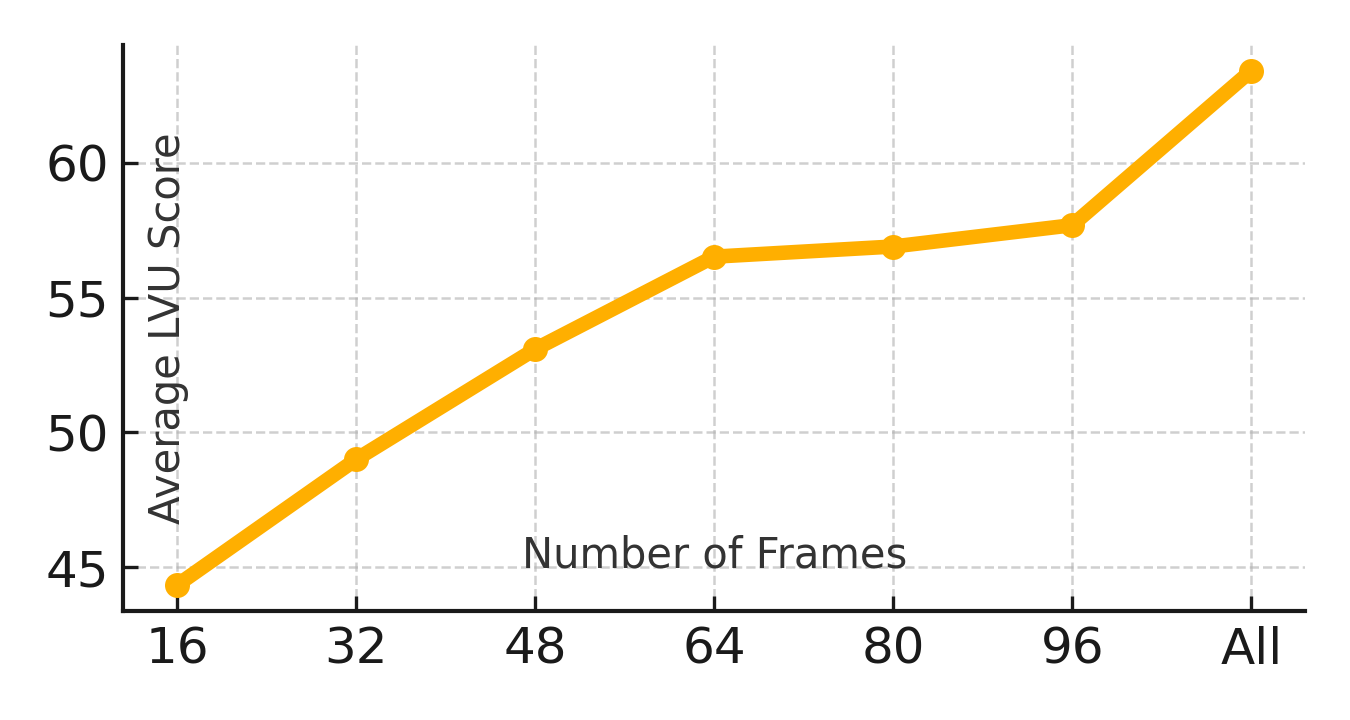
\includegraphics[width=1.\linewidth]{figures/lvu_performance.png}
  \caption{Average performance of LVU benchmark rises monotonically as the frame count increases.}
  \label{fig:lvu_func_len}
\end{figure}

\section{Short-Video Performance} 
\label{app:short_video_perf}

Our approach preserves performance on short-video understanding tasks. Specifically, we preserve the accuracy of LanguageBind on Kinetics-400 (600)~\cite{Kay2017TheKH}.
We achieved 78.2\% on K400 and 79.1\% on K600 compared to 77.6\% and 79.5\% in LanguageBind. 


\section{Additional Interpretable Predictions Results}
\label{app:interpretable_pred}

In Fig.~\ref{fig:interp_res_app}, we attach additional examples of the interpretable predictions experiment from \cref{sec:exp_interpretabitlity}.

\section{Additional Related Work}
\label{app:related}

\paragraph{Short-video understanding methods.} Numerous models have been proposed for short-video understanding, achieving remarkable performance on tasks such as action recognition \cite{arnab2021vivit}, video classification \cite{fan2021multiscale}, text-video retrieval \cite{luo2021clip4clip}, video captioning \cite{yang2021just}, and video question answering \cite{lei2021less}. Multimodal models like CLIP \cite{radford2021learning}, InternVideo \cite{Wang2024InternVideo2SV}, and LanguageBind \cite{zhu2024languagebind} have demonstrated strong capabilities in aligning video and language representations. In this work, we leverage the output embedding of these models to learn long-video representations. 

\begin{figure*}[ht]
    \centering
    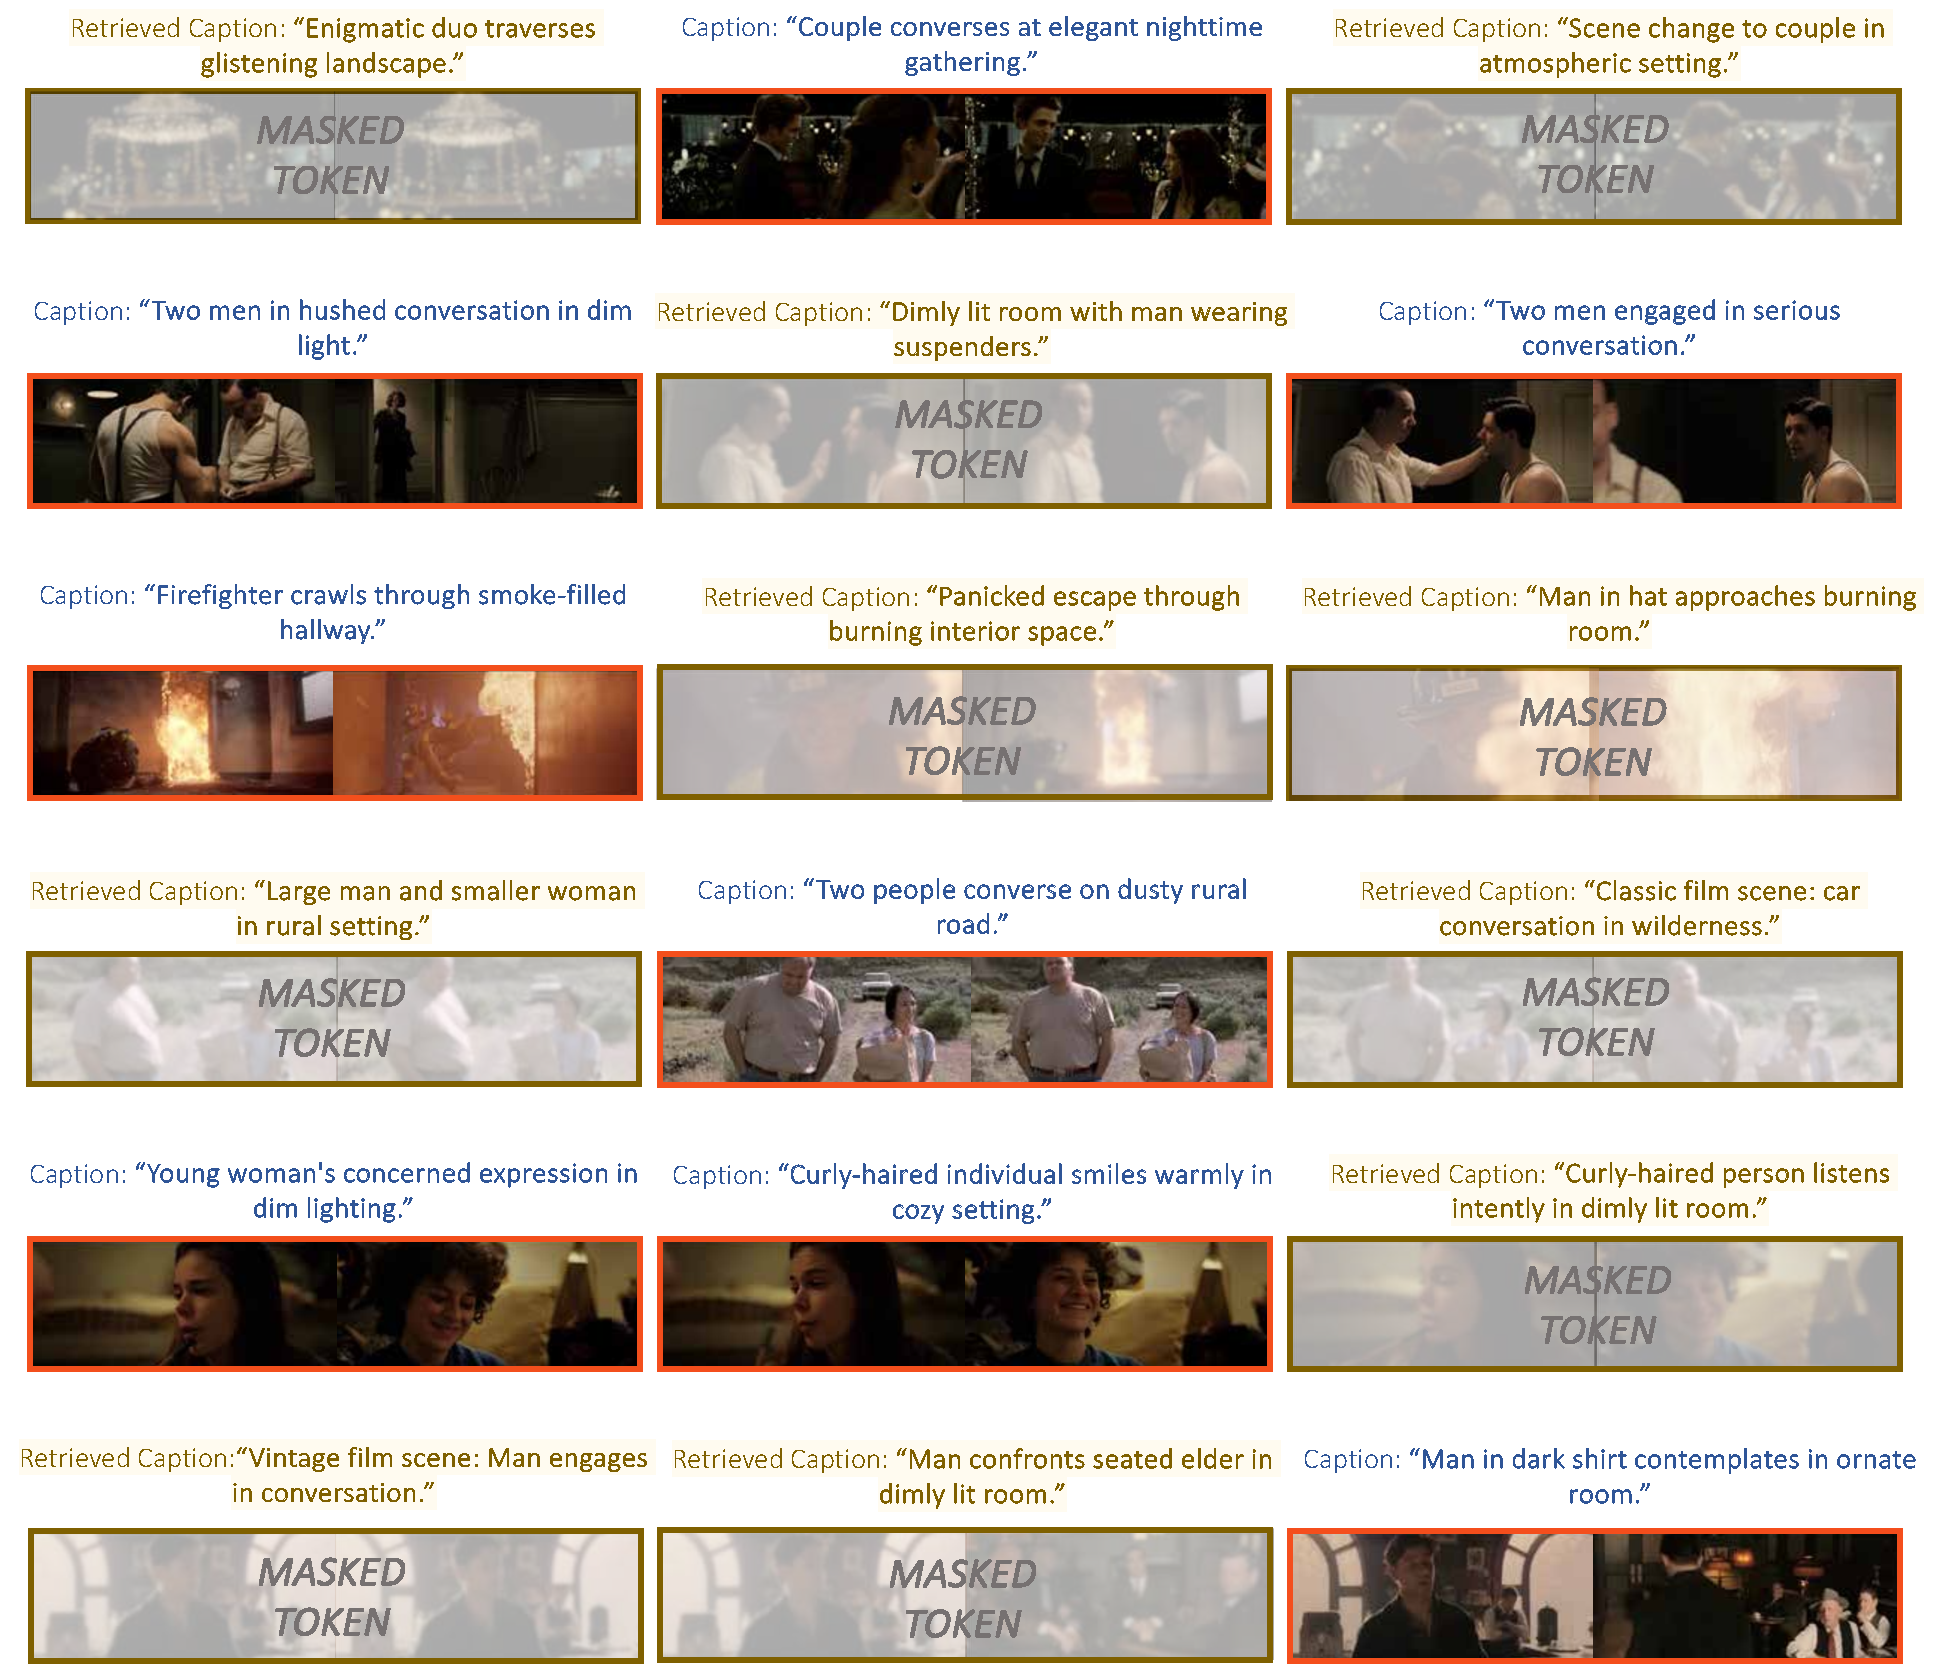
\includegraphics[width=1.\textwidth]{figures/interp_results_app.pdf}
    \caption{\textbf{Interpretable predictions -- additional examples}: Each row visualizes three consecutive five-second segments. Above each segment, we show the original caption for the visible tokens and the retrieved caption for the reconstructed masked tokens. As shown, the model successfully reconstructs the semantic meaning of the masked embeddings, offering insight into the model's effectiveness and capabilities.}
    \label{fig:interp_res_app}
\end{figure*}

\paragraph{Long-video language understanding methods.} Several recent works have advanced the field of video understanding using large language models. Video-XL~\cite{shu2024video} and LongVLM~\cite{weng2024longvlm} both tackle the challenge of processing long-form videos, with Video-XL focusing on hour-scale video understanding and LongVLM proposing efficient mechanisms for extended video content. LongVILA~\cite{chen2024longvila} further contributes to this direction by scaling visual language models for long video comprehension. In the domain of efficient video processing, VoCo-LLaMA~\cite{ye2024voco} explores video compression using large language models, while LLaMA-VID~\cite{li2024llama} proposes a compact two-token representation for video content. SlowFast-LLaVA~\cite{xu2024slowfast} provides a training-free baseline approach for video large language models. Addressing temporal aspects, TimeChat~\cite{ren2024timechat} develops time-sensitive capabilities for video understanding, while LITA~\cite{huang2024lita} focuses on precise temporal localization within videos. In contrast to these works that focus on video-language integration, we explore long-video masked-embedding autoencoders in long-form video classification tasks and aim to find effective representation learning methods specifically designed for long-form videos.
